\chapter{Titration Methods and Curves}\label{ch:b1:titration-methods}

A pharmacist receives a batch of vitamin C tablets labelled
\qty{500}{mg} and must certify, before they are sold, that each holds
what the label says. She will not weigh the vitamin directly: it is
mixed with binders and fillers. She will titrate it --- let it react with
a reagent of known concentration, measure the volume needed, and compute
the amount. Which reaction, how to see its end, and how sure the result
is: these are the questions of this chapter, which brings the equilibria
of the last five chapters to the laboratory bench.

\begin{recall}
The school volume (grades 11 and 12) titrated acids by bases with a
colour change, followed \omterm{def:b1:titration-methods:titration}{titrations} with a pH meter and a conductivity
meter, and used the \omterm{def:b1:titration-methods:titration}{equivalence} relation $C_AV_A = C_BV_B$. The
predominant-reaction method is in \cref{ch:b1:predominant-reaction};
precipitation, complexation and redox equilibria in
\cref{ch:b1:precipitation,ch:b1:complexation,ch:b1:nernst}.
\end{recall}

\begin{omfigure}
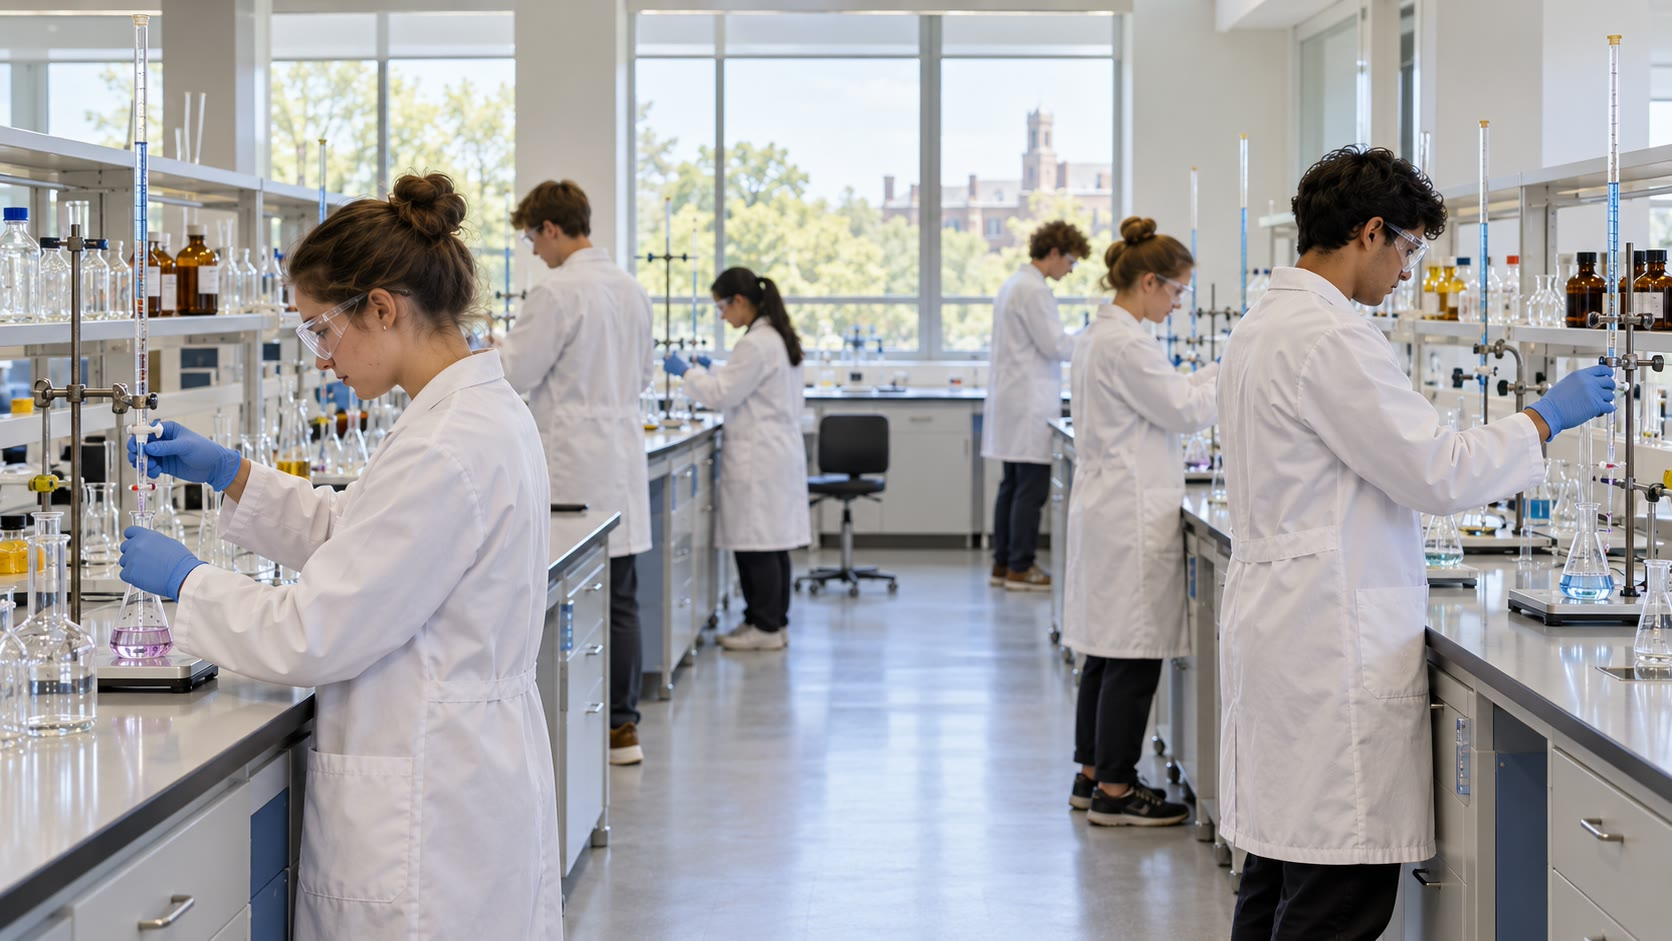
\includegraphics[width=0.66\linewidth]{images/book2/ai/b1-15-teaching-lab.jpg}

{\small A teaching laboratory: a burette, a conical flask on a magnetic
stirrer, gloves and goggles. A \omterm{def:b1:titration-methods:titration}{titration} is the most common quantitative
measurement in chemistry.}
\end{omfigure}

\section{Titration and equivalence}

\begin{definition}[Titration, equivalence]\label{def:b1:titration-methods:titration}
A \emph{titration}\index{titration} determines the amount of a species,
the \emph{analyte}\index{analyte}, by a reaction with a reagent of known
concentration, the \emph{titrant}\index{titrant}, added progressively. The
reaction must be single, \omterm{def:b1:extent-q-and-k:quantitative}{quantitative} ($K$ large) and fast. The
\emph{equivalence}\index{equivalence} is reached when titrant and analyte
have been brought together in the stoichiometric proportions of the
reaction; the volume added then is the equivalence volume, and the point
of the titration curve at that volume is the \emph{equivalence
point}\index{equivalence point}. The volume at which the experimenter
stops, seeing a colour change or a break in a curve, is the \emph{end
point}\index{end point}; a good method makes it coincide with the
equivalence.
\end{definition}

\begin{proposition}[Equivalence relation]\label{prop:b1:titration-methods:equivalence}
For a \omterm{def:b1:titration-methods:titration}{titration} reaction $a\,\mathrm{A} + b\,\mathrm{B} \to \cdots$, with
\omterm{def:b1:titration-methods:titration}{analyte} A ($n_A$ mol) and \omterm{def:b1:titration-methods:titration}{titrant} B at concentration $C_B$, the
\omterm{def:b1:titration-methods:titration}{equivalence} volume satisfies
\[
  \frac{n_A}{a} = \frac{C_B V_{\mathrm{eq}}}{b} .
\]
\end{proposition}

\begin{proof}
Let $x$ be the extent after adding $V$ of \omterm{def:b1:titration-methods:titration}{titrant}. Before \omterm{def:b1:titration-methods:titration}{equivalence} B
is limiting and, the reaction being \omterm{def:b1:extent-q-and-k:quantitative}{quantitative}, $x = C_BV/b$; after it,
A is limiting and $x = n_A/a$. The \omterm{def:b1:titration-methods:titration}{equivalence} is the volume where both
are used up together, $n_A - ax = 0$ and $C_BV - bx = 0$: eliminating $x$
gives the relation.
\end{proof}

\section{Direct and indirect titrations}

\begin{definition}[Kinds of titration]\label{def:b1:titration-methods:kinds}
In a \emph{direct titration}\index{direct titration} the \omterm{def:b1:titration-methods:titration}{titrant} reacts
with the \omterm{def:b1:titration-methods:titration}{analyte} itself. In a \emph{back titration}\index{back titration}
a known excess of a reagent is added to the \omterm{def:b1:titration-methods:titration}{analyte}, and the excess left
is titrated. When a solution contains several \omterm{def:b1:titration-methods:titration}{analytes} that react in
turn with the \omterm{def:b1:titration-methods:titration}{titrant}, they are measured by \emph{successive
titrations}\index{successive titrations}, one \omterm{def:b1:titration-methods:titration}{equivalence} after another;
when they react together and give a single \omterm{def:b1:titration-methods:titration}{equivalence}, by a
\emph{simultaneous titration}\index{simultaneous titration}, which gives
only their sum.
\end{definition}

\begin{method}[Back titration]\label{met:b1:titration-methods:back-titration}
Use it when the direct reaction is slow, when the \omterm{def:b1:titration-methods:titration}{analyte} is unstable or
volatile, or when no indicator fits the direct reaction.
\begin{enumerate}
  \item Add a known amount $n_R$ of reagent R, in excess, and let it react
        completely with the \omterm{def:b1:titration-methods:titration}{analyte} A ($\alpha\,\mathrm{A} + \rho\,\mathrm{R}$).
  \item Titrate the excess R with a \omterm{def:b1:titration-methods:titration}{titrant} T ($\rho'\,\mathrm{R} +
        \tau\,\mathrm{T}$) to the \omterm{def:b1:titration-methods:titration}{equivalence} volume $V_T$.
  \item Compute $n_{R,\text{excess}} = \frac{\rho'}{\tau}C_TV_T$, then
        $n_A = \frac{\alpha}{\rho}(n_R - n_{R,\text{excess}})$.
\end{enumerate}
\end{method}

The weekend problem titrates vitamin C this way: ascorbic acid reduces
an excess of iodine, and the iodine left is titrated by thiosulfate.

\section{pH-metric titrations and indicators}

\begin{omfigure}
\begin{tikzpicture}[font=\small]
  \pic at (0,0) {stirrer};
  \pic at (0,0.18) {beaker={0.55}{omDef!14}};
  \pic at (0.2,2.45) {burette={0.75}{white}};
  \pic at (-0.45,0.45) {probe};
  \pic (m) at (-2.6,3.2) {meter={pH}};
  \draw[thick] (-0.45,3.45) to[out=90, in=0] (m-b);
  \node[anchor=west] at (0.65,6.2) {burette: NaOH, \qty{0.100}{mol/L}};
  \node[anchor=west] at (1.0,1.0) {acid, $V_0 = \qty{10.0}{mL}$, diluted};
  \draw[<-, omProp, thick] (1.2,-0.25) -- (1.8,-0.25) node[anchor=west, text=black] {magnetic stirrer};
  \draw[<-, omProp, thick] (-0.62,2.4) -- (-1.5,2.0) node[anchor=east, text=black] {combined electrode};
\end{tikzpicture}

{\small A pH-metric \omterm{def:b1:titration-methods:titration}{titration}. The combined glass electrode measures the
pH after each addition from the burette; the stirrer mixes the solution.
The electrode is calibrated beforehand with two \omterm{def:b1:predominant-reaction:buffer}{buffer solutions}.}
\end{omfigure}

\begin{omfigure}
\begin{tikzpicture}
\begin{axis}[name=s,
  width=0.5\linewidth, height=5.6cm, xmin=0, xmax=20, ymin=0, ymax=14,
  axis x line=bottom, axis y line=left, xlabel={$V$ (mL)}, ylabel={pH},
  xtick={0,5,10,15,20}, ytick={0,2,4,6,8,10,12,14},
  tick label style={font=\small}, label style={font=\small}]
\addplot[omDef, very thick] table[x=V, y=pH] {figdata/out/bachelor-1-titration-curves-strong.dat};
\addplot[omProp, thick] table[x=V, y=pH] {figdata/out/bachelor-1-titration-curves-weak.dat};
\node[font=\scriptsize, omDef, anchor=south west] at (axis cs:6,0.2) {\ce{HCl}};
\node[font=\scriptsize, omProp, anchor=west] at (axis cs:0.4,6.4) {\ce{CH3COOH}};
\draw[dotted] (axis cs:5,0) -- (axis cs:5,4.76) -- (axis cs:0,4.76);
\node[font=\scriptsize, anchor=north] at (axis cs:2.5,4.7) {$\mathrm{p}K_a$};
\end{axis}
\begin{axis}[at={(s.east)}, anchor=west, xshift=1.2cm,
  width=0.5\linewidth, height=5.6cm, xmin=0, xmax=20, ymin=0, ymax=14,
  axis x line=bottom, axis y line=left, xlabel={$V$ (mL)}, ylabel={pH},
  xtick={0,5,10,15,20}, ytick={0,2,4,6,8,10,12,14},
  tick label style={font=\small}, label style={font=\small}]
\addplot[omMeth, very thick] table[x=V, y=pH] {figdata/out/bachelor-1-titration-curves-mixture.dat};
\node[font=\scriptsize, anchor=west, align=left] at (axis cs:10.8,6.0) {\ce{HCl} + \ce{CH3COOH}\\ two equivalences};
\end{axis}
\end{tikzpicture}

{\small Left: \qty{10.0}{mL} of hydrochloric acid and of ethanoic acid,
both at \qty{0.100}{mol/L}, titrated by sodium hydroxide at
\qty{0.100}{mol/L}. The \omterm{def:b1:predominant-reaction:strong-acid}{weak acid} has a buffer region with pH $=
\mathrm{p}K_a$ at \omterm{def:b1:titration-methods:titration}{half-equivalence} and an \omterm{def:b1:titration-methods:titration}{equivalence point} at pH 8.73.
Right: a mixture, \qty{0.050}{mol/L} of each acid: the \omterm{def:b1:predominant-reaction:strong-acid}{strong acid} is
titrated first (\omterm{def:b1:titration-methods:titration}{equivalence} at \qty{5}{mL}), then the weak one
(\qty{10}{mL}).}
\end{omfigure}

\begin{proposition}[Half-equivalence of a weak acid]\label{prop:b1:titration-methods:half-equivalence}
When a \omterm{def:b1:predominant-reaction:strong-acid}{weak acid} HA is titrated by a \omterm{def:b1:predominant-reaction:strong-acid}{strong base}, at \omterm{def:b1:titration-methods:titration}{half-equivalence}
$\mathrm{pH} = \mathrm{p}K_a$, provided that the acid is not too strong
nor too dilute ($\mathrm{p}K_a$ roughly between 4 and 10 at
\qty{0.1}{mol/L}).
\end{proposition}

\begin{proof}
At \omterm{def:b1:titration-methods:titration}{half-equivalence} the \omterm{def:b1:extent-q-and-k:quantitative}{quantitative reaction} \ce{HA + OH- -> A- + H2O}
has converted half of HA: $[\mathrm{HA}] = [\mathrm{A^-}]$, and the
Henderson relation gives $\mathrm{pH} = \mathrm{p}K_a$. The condition
ensures that the reaction of HA with water and that of $\mathrm{A^-}$
with water do not change those amounts appreciably.
\end{proof}

\begin{proposition}[pH at the equivalence of a weak acid]\label{prop:b1:titration-methods:ph-at-equivalence}
At the \omterm{def:b1:titration-methods:titration}{equivalence} of a \omterm{def:b1:predominant-reaction:strong-acid}{weak acid} ($\mathrm{p}K_a$) by a \omterm{def:b1:predominant-reaction:strong-acid}{strong base}, the
solution is the conjugate base at concentration $C'$ (after dilution), and
\[
  \mathrm{pH} = \tfrac12(\mathrm{p}K_e + \mathrm{p}K_a + \log C') .
\]
\end{proposition}

\begin{proof}
The \omterm{def:b1:predominant-reaction:predominant-reaction}{predominant reaction} of the base with water,
\ce{A- + H2O <=> HA + OH-}, has $K = K_e/K_a$; with little base
converted, $[\ce{OH-}] = \sqrt{KC'}$ (\cref{prop:b1:predominant-reaction:ph-formulas}),
whence the result. For ethanoic acid, $C' = \qty{0.050}{mol/L}$:
$\frac12(14.00 + 4.76 - 1.30) = 8.73$.
\end{proof}

\begin{proposition}[Successive titrations]\label{prop:b1:titration-methods:successive}
Two acids titrated by the same base give separate \omterm{def:b1:titration-methods:titration}{equivalences}, each to
better than \qty{1}{\percent}, if their $\mathrm{p}K_a$ differ by at least 4.
\end{proposition}

\begin{proof}
At the first \omterm{def:b1:titration-methods:titration}{equivalence}, the reaction of the base $\mathrm{A_1^-}$ with
the second acid $\mathrm{HA_2}$, $\mathrm{A_1^-} + \mathrm{HA_2}
\rightleftharpoons \mathrm{HA_1} + \mathrm{A_2^-}$, has $K = 10^{\mathrm{p}K_1 - \mathrm{p}K_2}$.
Starting from equal amounts, the fraction $x$ of the second acid already
titrated satisfies $x^2/(1 - x)^2 = K$; for $x \leqslant 0.01$, $K
\leqslant 10^{-4}$, that is $\mathrm{p}K_2 - \mathrm{p}K_1 \geqslant 4$.
\end{proof}

Phosphoric acid (2.15, 7.21, 12.34) gives two clear \omterm{def:b1:titration-methods:titration}{equivalences}; the
third is lost in the water of the base. Ethanoic acid mixed with
hydrochloric acid (right of the figure) is titrated after it, the \omterm{def:b1:predominant-reaction:strong-acid}{strong
acid} being in effect a $\mathrm{p}K_a$ below 0.

\begin{method}[Locating an equivalence on a curve]\label{met:b1:titration-methods:derivative}
\begin{enumerate}
  \item Derivative: compute $\Delta\mathrm{pH}/\Delta V$ between
        successive points; the \omterm{def:b1:titration-methods:titration}{equivalence} is at its maximum.
  \item Tangents: draw two parallel tangents to the curve on each side of
        the jump, and the parallel equidistant from them; it cuts the
        curve at the \omterm{def:b1:titration-methods:titration}{equivalence point}.
\end{enumerate}
\end{method}

\begin{method}[Tangents, by computation]\label{met:b1:titration-methods:tangents}
For a curve recorded by computer, fit the points of each side of the
jump with a smooth function and take the inflection point; for a
symmetric jump (\omterm{def:b1:predominant-reaction:strong-acid}{strong acid}, \omterm{def:b1:predominant-reaction:strong-acid}{strong base}) the midpoint of the jump at pH
7 is the \omterm{def:b1:titration-methods:titration}{equivalence point}.
\end{method}

\begin{definition}[Colour indicator, turning zone]\label{def:b1:titration-methods:indicator}
A \emph{colour indicator}\index{colour indicator} is a weak acid--base
pair HIn/In$^-$ whose two forms have different colours. Its colour changes
over the \emph{turning zone}\index{turning zone}, the pH range where
neither form clearly dominates, about $\mathrm{p}K_{a}(\mathrm{HIn}) \pm 1$.
\end{definition}

\begin{omfigure}
\begin{tabular}{lccl}
\hline
indicator & $\mathrm{p}K_a$ & \omterm{def:b1:titration-methods:indicator}{turning zone} & colours (acid / base) \\
\hline
methyl orange & 3.5 & 2.5--4.5 & red / yellow \\
methyl red & 4.8 & 3.8--5.8 & red / yellow \\
phenol red & 7.9 & 6.9--8.9 & yellow / red \\
thymol blue (second change) & 9.2 & 8.2--10.2 & yellow / blue \\
\hline
\end{tabular}

\smallskip
{\small Four indicators, $\mathrm{p}K_a$ from a critical compilation of
\omterm{def:b1:complexation:formation-constant}{dissociation constants}; the \omterm{def:b1:titration-methods:indicator}{turning zones} are $\mathrm{p}K_a \pm 1$.}
% ledger: pka:methylorange, pka:methylred, pka:phenolred, pka:thymolblue2
\end{omfigure}

\begin{method}[Choosing an indicator]\label{met:b1:titration-methods:choose-indicator}
Choose an indicator whose \omterm{def:b1:titration-methods:indicator}{turning zone} lies inside the vertical jump of
the curve, as close as possible to the pH at \omterm{def:b1:titration-methods:titration}{equivalence}. \omterm{def:b1:predominant-reaction:strong-acid}{Strong acid} by
\omterm{def:b1:predominant-reaction:strong-acid}{strong base} (jump 3.3 to 10.7 for $\pm\qty{0.1}{mL}$ here): any of the
four. Ethanoic acid (\omterm{def:b1:titration-methods:titration}{equivalence} 8.73): phenol red or thymol blue; methyl
orange would change colour long before the \omterm{def:b1:titration-methods:titration}{equivalence}.
\end{method}

\section{Potentiometric titrations}

\begin{definition}[Potentiometric titration]\label{def:b1:titration-methods:potentiometric}
A \emph{potentiometric titration}\index{potentiometric titration}
follows the potential of an electrode in the solution against a
\omterm{def:b1:nernst:reference-electrode}{reference electrode}, for a redox (platinum wire), precipitation (silver
wire) or complexation \omterm{def:b1:titration-methods:titration}{titration}.
\end{definition}

\begin{proposition}[Remarkable points of a redox titration]\label{prop:b1:titration-methods:potentiometric-points}
For the \omterm{def:b1:titration-methods:titration}{titration} of $\mathrm{Red_1}$ by $\mathrm{Ox_2}$ with
$n_2\,\mathrm{Red_1} + n_1\,\mathrm{Ox_2} \to n_2\,\mathrm{Ox_1} +
n_1\,\mathrm{Red_2}$ (couples of $n_1$ and $n_2$ electrons), $E(V_{\mathrm{eq}}/2) = E^\circ_1$, $E(2V_{\mathrm{eq}}) =
E^\circ_2$, and at \omterm{def:b1:titration-methods:titration}{equivalence}
\[
  E_{\mathrm{eq}} = \frac{n_1E^\circ_1 + n_2E^\circ_2}{n_1 + n_2},
\]
for couples whose \omterm{def:b1:nernst:couple}{half-equations} involve no other species (or at a pH
that keeps the extra terms fixed).
\end{proposition}

\begin{proof}
At \omterm{def:b1:titration-methods:titration}{half-equivalence} half of $\mathrm{Red_1}$ is oxidised:
$[\mathrm{Ox_1}] = [\mathrm{Red_1}]$ and the \omterm{thm:b1:nernst:nernst}{Nernst equation} of couple 1
gives $E^\circ_1$. At $2V_{\mathrm{eq}}$ as much $\mathrm{Ox_2}$ is in excess as
was reduced: $[\mathrm{Ox_2}] = [\mathrm{Red_2}]$, $E = E^\circ_2$. At
\omterm{def:b1:titration-methods:titration}{equivalence}, multiply the \omterm{thm:b1:nernst:nernst}{Nernst equation} of couple 1 by $n_1$ and that of
couple 2 by $n_2$ and add; the stoichiometry makes
$[\mathrm{Ox_1}]/[\mathrm{Red_1}] \cdot [\mathrm{Ox_2}]/[\mathrm{Red_2}] = 1$
(the amounts of $\mathrm{Red_1}$ and $\mathrm{Ox_2}$ left are in the same
ratio as the products), so the logarithms cancel.
\end{proof}

For iron(II) by permanganate in \qty{1}{mol/L} acid, $n_1 = 1$ and $n_2 =
5$: $E_{\mathrm{eq}} = (0.77 + 5 \times 1.51)/6 = 1.39$~V. The jump, from
about 0.8 to 1.5~V, is so large that the \omterm{def:b1:titration-methods:titration}{end point} is sharp; in practice
permanganate is its own indicator, its violet colour persisting at the
first drop in excess.

\begin{omfigure}
\begin{tikzpicture}
\begin{axis}[name=p,
  width=0.5\linewidth, height=5.6cm, xmin=0, xmax=20, ymin=0.6, ymax=1.6,
  axis x line=bottom, axis y line=left, xlabel={$V$ (mL)}, ylabel={$E$ (V)},
  xtick={0,5,10,15,20},
  tick label style={font=\small}, label style={font=\small}]
\addplot[omDef, very thick] table[x=V, y=E] {figdata/out/bachelor-1-titration-curves-potentiometric.dat};
\draw[dotted] (axis cs:5,0.6) -- (axis cs:5,0.77) -- (axis cs:0,0.77);
\draw[dotted] (axis cs:10,0.6) -- (axis cs:10,1.39) -- (axis cs:0,1.39);
\node[font=\scriptsize, anchor=south west] at (axis cs:0.2,0.77) {0.77};
\node[font=\scriptsize, anchor=south west] at (axis cs:0.2,1.39) {1.39};
\end{axis}
\begin{axis}[at={(p.east)}, anchor=west, xshift=1.2cm,
  width=0.5\linewidth, height=5.6cm, xmin=0, xmax=20, ymin=0, ymax=4.6,
  axis x line=bottom, axis y line=left, xlabel={$V$ (mL)},
  ylabel={$\kappa$ (mS/cm)}, xtick={0,5,10,15,20},
  tick label style={font=\small}, label style={font=\small}]
\addplot[omProp, very thick] table[x=V, y=kappa] {figdata/out/bachelor-1-titration-curves-conductimetric.dat};
\draw[dotted] (axis cs:10,0) -- (axis cs:10,1.15);
\end{axis}
\end{tikzpicture}

{\small Left: \omterm{def:b1:titration-methods:potentiometric}{potentiometric titration} of \qty{10.0}{mL} of iron(II) at
\qty{0.100}{mol/L} by permanganate at \qty{0.0200}{mol/L} in
\qty{1}{mol/L} acid (platinum electrode, potential against the hydrogen
electrode). Right: conductimetric \omterm{def:b1:titration-methods:titration}{titration} of \qty{100}{mL} of
hydrochloric acid at \qty{0.0100}{mol/L} by sodium hydroxide at
\qty{0.100}{mol/L}; the \omterm{def:b1:titration-methods:titration}{equivalence} is at the intersection of two
straight lines.}
% ledger: lam:H+, lam:OH-, lamsalt:HCl, lamsalt:NaCl (conductivities in figdata/bachelor-1/titration-curves.py)
\end{omfigure}

\section{Conductimetric, complexometric and precipitation titrations}

\begin{definition}[Molar ionic conductivity]\label{def:b1:titration-methods:conductivity}
The conductivity $\kappa$ of a solution (in \unit{S/m}) measures how well
it carries current through the motion of its ions. The \emph{molar ionic
conductivity}\index{molar ionic conductivity} $\lambda_i$ of an ion is its
contribution per mole per unit volume; its value at infinite dilution,
$\lambda_i^\circ$, is a constant of the ion and the solvent at a given
temperature.
\end{definition}

\begin{proposition}[Kohlrausch's law]\label{prop:b1:titration-methods:kohlrausch}
In dilute solution, the conductivity is the sum of the contributions of
the ions,
\[
  \kappa = \sum_i \lambda_i^\circ c_i ,
\]
\emph{Kohlrausch's law}\index{Kohlrausch's law}; the molar conductivity of
a salt is the sum of those of its ions.
\end{proposition}

\admitted{\omterm{prop:b1:titration-methods:kohlrausch}{Kohlrausch's law} expresses that dilute ions move
independently; its limits at higher concentration are studied in the
Year~2 volume. We use it here as an experimental law.}

\begin{proposition}[Slopes of a conductimetric titration]\label{prop:b1:titration-methods:conductimetric-slopes}
When a \omterm{def:b1:predominant-reaction:strong-acid}{strong acid} H$^+$X$^-$ is titrated by a \omterm{def:b1:predominant-reaction:strong-acid}{strong base}
Na$^+$OH$^-$ in a large volume (dilution neglected), the conductivity
varies linearly with the volume added, with slope proportional to
$\lambda^\circ(\ce{Na+}) - \lambda^\circ(\ce{H+}) < 0$ before
\omterm{def:b1:titration-methods:titration}{equivalence} and to $\lambda^\circ(\ce{Na+}) + \lambda^\circ(\ce{OH-}) > 0$
after.
\end{proposition}

\begin{proof}
Before \omterm{def:b1:titration-methods:titration}{equivalence} each mole of hydroxide added removes one mole of
\ce{H+} (\ce{H+ + OH- -> H2O}) and brings one mole of \ce{Na+}; after
\omterm{def:b1:titration-methods:titration}{equivalence} it adds one \ce{Na+} and one \ce{OH-}. \ce{X-} is unchanged.
By \omterm{prop:b1:titration-methods:kohlrausch}{Kohlrausch's law} the conductivity changes by those combinations of
$\lambda^\circ$ times the amount added divided by the (fixed) volume.
\end{proof}

From the limiting conductivities, $\lambda^\circ(\ce{H+}) =
\qty{349.8}{S.cm^2/mol}$ and $\lambda^\circ(\ce{OH-}) = 198.3$, and those
of the salts \ce{HCl} (426) and \ce{NaCl} (126.5), \omterm{prop:b1:titration-methods:kohlrausch}{Kohlrausch's law} gives
$\lambda^\circ(\ce{Cl-}) = 426 - 349.8 = 76.2$ and $\lambda^\circ(\ce{Na+}) =
126.5 - 76.2 = 50.3$~\unit{S.cm^2/mol}. The hydrogen and hydroxide ions
conduct far better than the others: the curve is a sharp V.

Complexometric \omterm{def:b1:titration-methods:titration}{titrations} use edta: at pH 10 (ammonia buffer) calcium
and magnesium react with it \omterm{def:b1:extent-q-and-k:quantitative}{quantitatively} (conditional constants of
\cref{ch:b1:complexation}), and an indicator that is itself a weak
complexing agent of the metal changes colour when edta takes the last
metal ions from it --- the \omterm{def:b1:titration-methods:titration}{titration} of water hardness. Precipitation
\omterm{def:b1:titration-methods:titration}{titrations} use silver ions: chloride is titrated by silver nitrate with
chromate as the indicator (\cref{exo:b1:precipitation:8}), or followed
with a silver electrode (\cref{ch:b1:nernst}). The precision of all these
results, set by the glassware and the \omterm{def:b1:titration-methods:titration}{end point}, is treated in
\cref{ch:b1:lab-techniques-1}.

\section{Exercises}

\begin{exercise}[$\star$]\label{exo:b1:titration-methods:1}
\qty{20.0}{mL} of a sodium hydroxide solution need \qty{12.4}{mL} of
hydrochloric acid at \qty{0.100}{mol/L}. Write the reaction, its constant,
and compute the concentration of the base.
\end{exercise}

\begin{exercise}[$\star$]\label{exo:b1:titration-methods:2}
Which indicator of the table suits the \omterm{def:b1:titration-methods:titration}{titration} of ammonia (\qty{0.10}{mol/L},
$\mathrm{p}K_a = 9.25$) by hydrochloric acid at \qty{0.10}{mol/L}? Compute
the pH at \omterm{def:b1:titration-methods:titration}{equivalence} first.
\end{exercise}

\begin{exercise}[$\star$]\label{exo:b1:titration-methods:3}
\qty{10.0}{mL} of iron(II) are titrated by permanganate at
\qty{0.0200}{mol/L}; the violet colour persists from \qty{12.6}{mL}.
Write the reaction and compute the concentration of iron(II).
\end{exercise}

\begin{exercise}[$\star$]\label{exo:b1:titration-methods:4}
A water sample of \qty{50.0}{mL} is titrated by edta at
\qty{0.0100}{mol/L} at pH 10; the \omterm{def:b1:titration-methods:titration}{equivalence} is at \qty{14.2}{mL}. Edta
reacts one to one with calcium and magnesium. Compute the total
concentration of these two ions. Is this a simultaneous or a successive
\omterm{def:b1:titration-methods:titration}{titration}?
\end{exercise}

\begin{exercise}[$\star\star$]\label{exo:b1:titration-methods:5}
For the \omterm{def:b1:titration-methods:titration}{titration} of \qty{10.0}{mL} of ethanoic acid at \qty{0.100}{mol/L}
by sodium hydroxide at \qty{0.100}{mol/L}, compute the pH at 0, 5.0, 10.0
and \qty{15.0}{mL} with the methods of \cref{ch:b1:predominant-reaction},
and compare with the curve of this chapter.
\end{exercise}

\begin{exercise}[$\star\star$]\label{exo:b1:titration-methods:6}
Show that a pH-metric \omterm{def:b1:titration-methods:titration}{titration} of phosphoric acid by sodium hydroxide
gives two jumps, and compute the pH at each \omterm{def:b1:titration-methods:titration}{equivalence} for an acid at
\qty{0.100}{mol/L} (\qty{10.0}{mL}, base \qty{0.100}{mol/L}). Why is there
no third jump?
\end{exercise}

\begin{exercise}[$\star\star$]\label{exo:b1:titration-methods:7}
A mixture of hydrochloric acid and ethanoic acid (\qty{10.0}{mL}) is
titrated by sodium hydroxide at \qty{0.100}{mol/L}: two \omterm{def:b1:titration-methods:titration}{equivalences}, at
\qty{6.2}{mL} and \qty{14.6}{mL}. Compute the two concentrations. What is
the pH halfway between the two \omterm{def:b1:titration-methods:titration}{equivalences}?
\end{exercise}

\begin{exercise}[$\star\star$]\label{exo:b1:titration-methods:8}
Compute the potential of the platinum electrode in the \omterm{def:b1:titration-methods:titration}{titration} of
iron(II) by permanganate (data of the chapter) at 2.0, 9.0, 11.0 and
\qty{20.0}{mL}.
\end{exercise}

\begin{exercise}[$\star\star$]\label{exo:b1:titration-methods:9}
Using \omterm{prop:b1:titration-methods:kohlrausch}{Kohlrausch's law} and the values of the chapter, compute the
conductivity of the titrated hydrochloric acid at 0, 10.0 and
\qty{20.0}{mL} of base (\qty{100}{mL} of acid at \qty{0.0100}{mol/L}, base
\qty{0.100}{mol/L}, dilution taken into account), and the two slopes.
\end{exercise}

\begin{exercise}[$\star\star\star$]\label{exo:b1:titration-methods:10}
Prove that the pH-metric curve of a \omterm{def:b1:predominant-reaction:strong-acid}{strong acid} titrated by a \omterm{def:b1:predominant-reaction:strong-acid}{strong base}
is symmetric about the \omterm{def:b1:titration-methods:titration}{equivalence point} when dilution is neglected,
and compute the size of the jump between $V_{\mathrm{eq}} \pm 0.1$~mL
for the \omterm{def:b1:titration-methods:titration}{titration} of the chapter. How does it change if all
concentrations are divided by 100?
\end{exercise}

\begin{exercise}[$\star\star\star$]\label{exo:b1:titration-methods:11}
Derive the equation of the potentiometric curve of iron(II) by
permanganate before and after the \omterm{def:b1:titration-methods:titration}{equivalence}, and check the three
remarkable points of \cref{prop:b1:titration-methods:potentiometric-points}.
How would the \omterm{def:b1:titration-methods:titration}{equivalence} potential change at pH 1?
\end{exercise}

\begin{exercise}[$\star\star\star$]\label{exo:b1:titration-methods:12}
Ammonium chloride (\qty{0.100}{mol/L}, $\mathrm{p}K_a = 9.25$) cannot be
titrated accurately by sodium hydroxide with an indicator. Explain from
the curve, then propose a \omterm{def:b1:titration-methods:kinds}{back titration}: excess sodium hydroxide, boil
off the ammonia, titrate the remaining hydroxide with hydrochloric acid.
Write the computation.
\end{exercise}

\section{Problem: How Much Vitamin C in the Tablet?}

\begin{problem}[{Weekend problem --- the reaction of iodine with ascorbic
acid, a back titration by thiosulfate, the computation of the result,
and its uncertainty, ending on the mass of ascorbic acid per tablet}]
\label{pb:b1:titration-methods:1}
A tablet is crushed and dissolved in water in a \qty{100.0}{mL}
volumetric flask. A \qty{10.00}{mL} aliquot is taken with a pipette, and
\qty{20.00}{mL} of iodine solution at \qty{0.0250}{mol/L} are added (excess). The
iodine left is titrated by sodium thiosulfate at \qty{0.0500}{mol/L} with
starch as the indicator: the blue colour vanishes at \qty{8.90}{mL}.
Ascorbic acid is \ce{C6H8O6} ($M = \qty{176.0}{g/mol}$); iodine oxidises
it to \ce{C6H6O6}. $E^\circ(\ce{I2}/\ce{I-}) = 0.53$~V,
$E^\circ(\ce{S4O6^2-}/\ce{S2O3^2-}) = 0.02$~V.

\medskip
\noindent\textbf{Part I --- The reactions.}
\begin{enumerate}
  \item Write the \omterm{def:b1:nernst:couple}{half-equation} of the couple \ce{C6H6O6}/\ce{C6H8O6}.
  \item Write the reaction of iodine with ascorbic acid.
  \item Give the \omterm{def:b1:nernst:oxidation-number}{oxidation number} of iodine in \ce{I2} and \ce{I-}.
  \item Write the reaction of iodine with thiosulfate and compute its
        constant.
  \item Starch gives a deep blue colour with iodine. Why does the colour
        vanish exactly at the \omterm{def:b1:titration-methods:titration}{equivalence} of the thiosulfate \omterm{def:b1:titration-methods:titration}{titration}?
  \item Ascorbic acid is slowly oxidised by the oxygen of air. Why does
        that argue for adding the iodine at once, in excess?
\end{enumerate}

\medskip
\noindent\textbf{Part II --- Why a \omterm{def:b1:titration-methods:kinds}{back titration}?}
\begin{enumerate}[resume]
  \item What would a \omterm{def:b1:titration-methods:kinds}{direct titration} of ascorbic acid by iodine require?
  \item Describe the \omterm{def:b1:titration-methods:kinds}{back titration} as the three steps of
        \cref{met:b1:titration-methods:back-titration}.
  \item Why must the iodine be in excess? Check it with the result.
  \item Why is the thiosulfate solution standardised shortly before use?
  \item The aliquot is \qty{10.00}{mL} of \qty{100.0}{mL}: what is the
        dilution factor?
  \item Which glassware delivers the \qty{20.00}{mL} of iodine solution?
\end{enumerate}

\medskip
\noindent\textbf{Part III --- The computation.}
\begin{enumerate}[resume]
  \item Compute the amount of iodine introduced.
  \item Compute the amount of thiosulfate used.
  \item Deduce the amount of iodine in excess.
  \item Deduce the amount of iodine that reacted with ascorbic acid.
  \item Compute the amount of ascorbic acid in the aliquot.
  \item Compute the amount, then the mass, of ascorbic acid in the
        tablet.
  \item Compare with the label (\qty{500}{mg}).
\end{enumerate}

\medskip
\noindent\textbf{Part IV --- How sure?}
The tolerances are: flask \qty{100.0 \pm 0.1}{mL}, pipettes
\qty{10.00 \pm 0.02}{mL} and \qty{20.00 \pm 0.03}{mL}, burette reading
$\pm\qty{0.05}{mL}$; the two concentrations are known to \qty{0.2}{\percent}.
\begin{enumerate}[resume]
  \item Express $n(\text{ascorbic acid})$ in the tablet as a function of the
        measured quantities.
  \item Which relative uncertainties enter the amount of iodine introduced
        and the amount in excess?
  \item Why does a difference of two amounts amplify the relative
        uncertainty?
  \item Combining the contributions as in \cref{ch:b1:lab-techniques-1}
        (quadratic sum), estimate the relative uncertainty of the result.
  \item Give the mass of ascorbic acid per tablet with its uncertainty, to
        two significant figures.
\end{enumerate}
\end{problem}
